\subsubsection{Fault Analysis }

We  compare the impact of losing $d$ machines using the following two approaches:
\begin{itemize}
\item The VM-centric approach (VC).  The replication degree of the backup storage 
is $r$ for regular content blocks and $r_c$ for CDS blocks where $r_c>r$. 
\item The VM-oblivious (VO) approach.
All chunk  blocks are treated uniformly and global comparison is conducted.
\end{itemize} 
 
When $d<r$, there is no loss of data in the snapshot storage.
When $d \ge r$, some of data blocks in the storage are loss, and we compute the number of VMs that could
suffer the loss of their snapshots.
We use the following parameters  during the analysis
\begin{itemize}
\item 	$V$ is the number of VMs. $m$ is the number of physical machines hosting the bakcup storage.
$d$ is the number of machines failed.
\item In the VC approach, $s_c$  of them in the backup storage
are shared by others with a zipf distribution. $(1-s_c)$ 
of them  is unique (nobody shares with them).
$L_c$ is the average number of VMs sharing a block (if it is in CDS for the VC approach.
$b_c$ is the number of shared blocks in VC.
\item In the VO approach, $s_o$ is the number of blocks shared.
$L_o$ is the average number of VMs sharing a block. 
\item $b$ is the  number of blocks stored in the storage after deduplication.
 \end{itemize}

The distribution of data blocks shared among VMs in VC follows a zipf distribution.
Given a VM block, the probability of being rank $x$ block is $P(x) = P(1) * x^{-\alpha}$
where $P(1)$ is the probability of being rank 1 most popular block.
Since $\sum P(x)= 1$, $P(1)= \frac{1}{\sum_1^{b_c} x^{-\alpha} }$.
Let $y$ be the number of VMs sharing rank $x$ block in VC, and  then  $y= V* P(x)$.

Thus the average number of VMs sharing a data block in the VC backup storage is:
\begin{equation}
%\begin{align}
\begin{split}
L_c& =  (1-s_c)*1 + s_c \sum_1^{b_c} P(x) * y \\
& =  (1-s_c)*1 + s_c \sum P(1)^2 *  x^{-2\alpha} *  V.
\end{split}
%\end{align}
\end{equation}

We can build a bipartite graph representing the association from unique data blocks
to their corresponding VMs. An association edge is  drawn  from a data block  to a VM 
if this block is used by this VM, 
The average incoming degree of VM nodes is equal to
the average outgoing degree of data blocks, which is $L_c$. 


\begin{figure}[htbp]
\centering
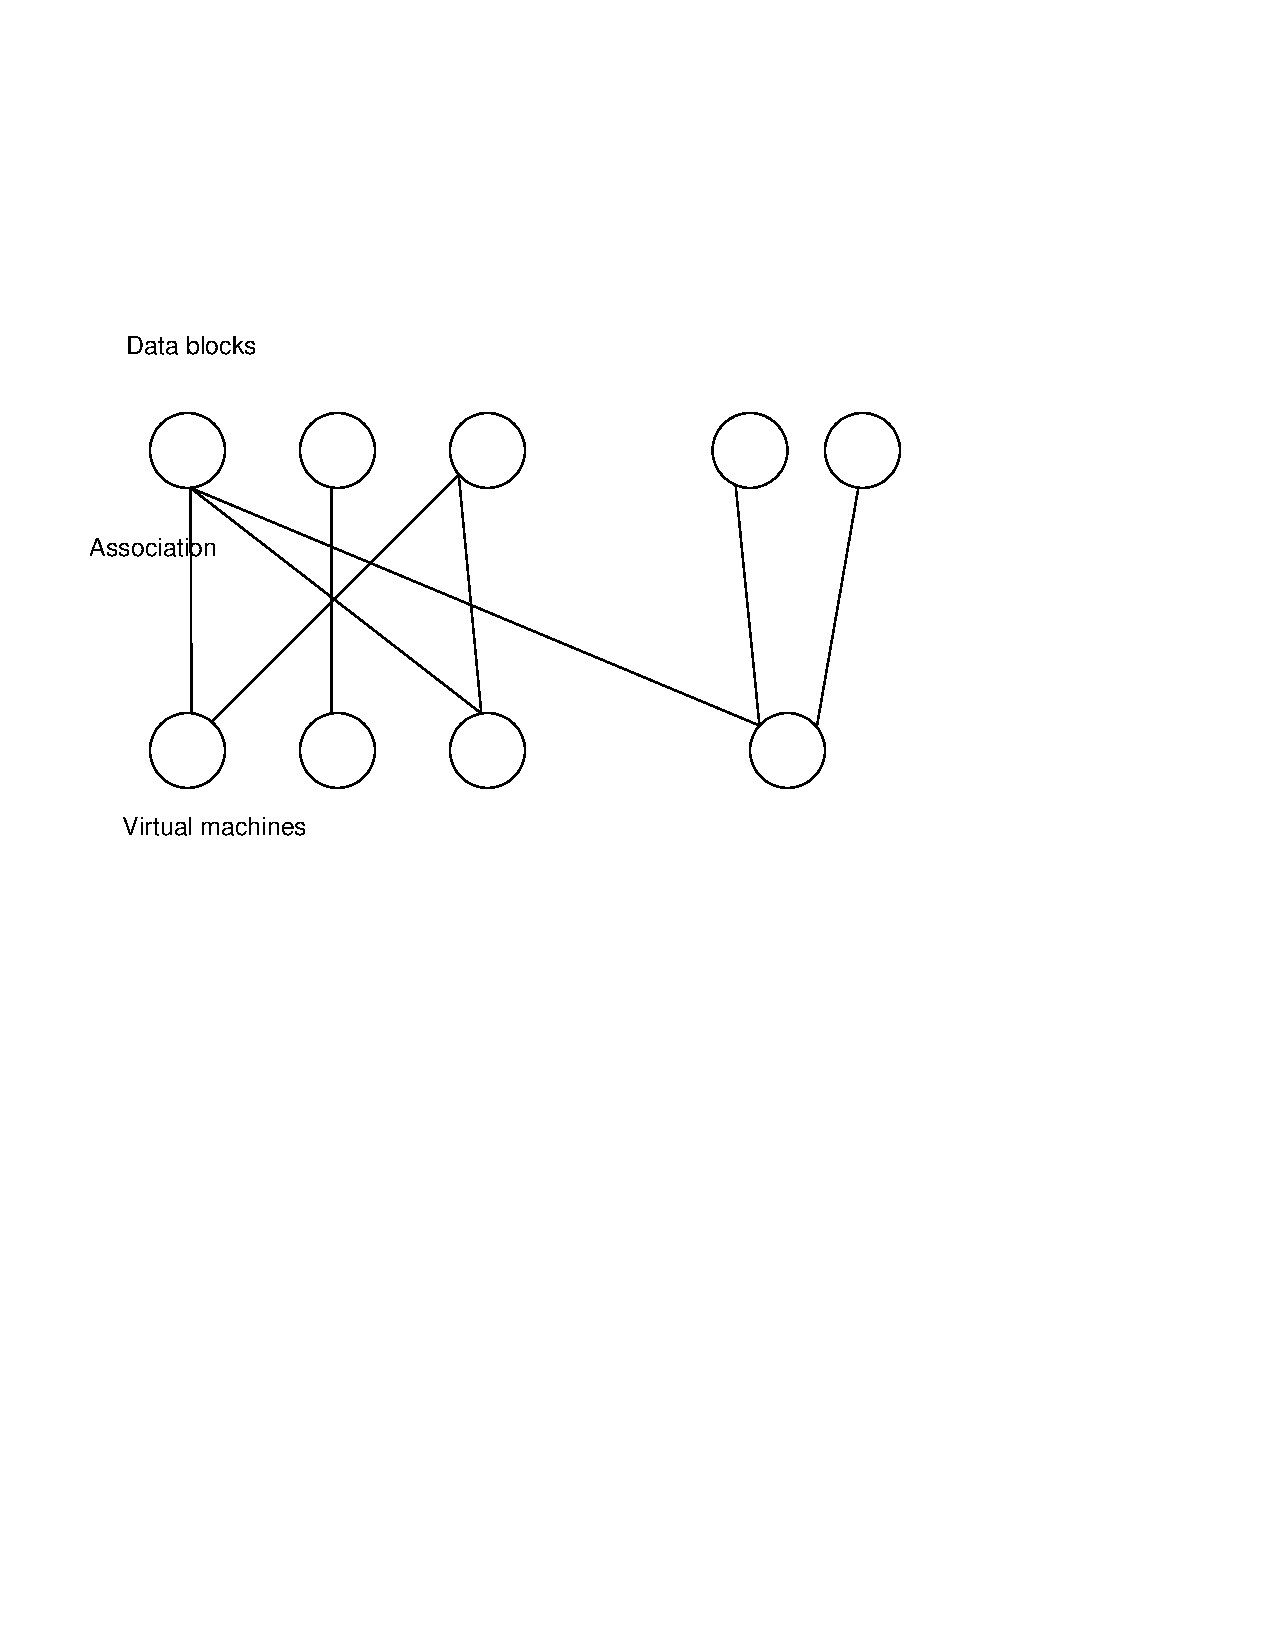
\includegraphics[width=0.45\textwidth]{shared.pdf}
\caption{Assoication of data blocks to VMs.}
\label{fig:shared}
\end{figure}


Under $d$ failed machines, the  expected number of VMs 
which suffer from data loss in VC is
\begin{multline}
%\begin{split}
 \sum_{1}^{V}  ( Probability (\mbox{ a VM fails)}) \\
= \sum_{1}^{V}  ( 1- Probability (\mbox{ a VM has no data loss)}) \\
= V ( 1-  Probability(\mbox{ A block has no data loss} )^{L_c} ).
%\end{split}
\end{multline}

\comments{
Prob(i-th block shared by (V-i+1) machines = X/i.
b
Sum (X/i) =1.      Thus       X= 1/ ln (V).
Length of sharing=  Probality(this block is shared with 1 VM) 1 + Probablity(this block shared by 2 VM) 2+..] =  X *V +X*(V-1)/2+ X*(V-2)/3 +..
=  X * sum (V-i+1)/I   for I from 1 to V.
=  (V+1) sum (X/i) . Sum(X) =  (V+1) -  X*V= V(1- 1/lnV) +1.
}

%Thus the number of VMs using a block =    $(1-s_c)  + s_c *L$.

When there are $d$ machines failed and the probability of
a block failure depends on if all replicas of this block reside in the failed machines.
When $r< d <r_c$,  only unshared data blocks can fail in VC. Then
%Probablity(\mbox { no loss for this  block}) = 1 - Probability (\mbox{ this block in d failed machiens})
\begin{multline}
%\begin{split}
Probability(\mbox{ A block has data loss})\\
= (1-s_c) (1- Probability (\mbox{ this block in d failed machines}))\\
= (1-s_c) (1- \frac{ \binom{d}{r}} { \binom{m}{r} }).
%\end{split}
\end{multline}
When $r_c \leq d$, shared data blocks in VC can have a loss. 
\[
Probability(\mbox{A block has data loss})
= 
(1-s_c) (1- \frac{ \binom{d}{r}} { \binom{m}{r} })
+ s_c (1- \frac{ \binom{r_c}{d}} { \binom{m}{r_c} }).
\]

By comparison, under $d$ failed machines, the  expected number of VMs 
which suffer from data loss in VO is
\[
V ( 1-  (1- \frac{ \binom{d}{r}} { \binom{m}{r} })^{L_o} ).
\]
where
\[
L_o = (1-s_o) + s_o \sum_1^b  P(1)^2 *  (x')^{-2\alpha'} *V.  
\]


\comments{
	=  sum _for_all_block(   Probablity (a block fails) *number of VM sharing this block ))
               = Probability(a block fails) * sum_for_all_blocks (numb of VM shared)
	= Probablity (a block fails) *b *aveageLengthVM
	= [ 1-  C(r, k) /C(n,r)] * b* [ 1+ s *V(1-1/ln V)]
  
----------------------------------------------------------------------       

For CDS model, 85% blocks are using the data from the same VM while upto 10% data is for CDS (we actually only use 5% perhaps).  Thus the overall speaking, at most 10% of data are shared.
Thus  for CDS approach,   the # VM failure caused by k machines is at most  [ 1-  C(r, k) /C(n,r)] * b* [ 1+ 0.10 *V(1-1/ln V)].
For original approach,  [ 1-  C(r, k) /C(n,r)] * b* [ 1+ 0.90 *V(1-1/ln V)].
For large V, the reliability improves by 9 times.
}
